\documentclass[11pt]{article}

\usepackage[margin=1in]{geometry}
\usepackage{amsmath}
\usepackage{amssymb}
\usepackage[titles]{tocloft}
\usepackage{graphicx}

\usepackage{tikz}
\usetikzlibrary{arrows.meta,positioning}

\title{SIST: The Sparse Inventory Service Twin}
\author{}
\date{\today}

\setlength{\parindent}{0pt}
\setlength{\parskip}{1\baselineskip}

\begin{document}

\begin{titlepage}
\maketitle

\begin{abstract}
SIST (Sparse Inventory Service Twin) is a single-user Bayesian generative model for businesses that sell services (and optionally retail SKUs) but only record inventory intermittently. From sparse stock snapshots, SIST infers a plausible latent ledger of service demand, retail demand, restocks, and adjustments, while adapting to drift, seasonality, promotions, and occasional change points.

The model is designed to work with minimal inputs (inventory reports), but can optionally incorporate low-effort signals such as prices, ranked lists of top services/SKUs, restock-included flags, service--SKU sharing masks, and stockout flags to improve identifiability.

Primary outputs are posterior inventory trajectories with uncertainty, demand-rate estimates and forecasts, stockout risk, and reorder policies (including safety stock and reorder points) under explicit service-level targets.
\end{abstract}

\vspace{1em}
\noindent\textbf{Keywords:} Bayesian inference; inventory reconstruction; stockout risk; demand drift; restocking policy; safety stock; reorder point.

\end{titlepage}

\tableofcontents
\newpage

\section{What SIST models}

\textbf{Scope.} SIST targets single-user settings where inventory is observed intermittently, direct sales logs may be missing, and operational decisions (stockout risk, reorder timing, safety stock) still need uncertainty-aware support.

\textbf{Contribution summary.}
\begin{enumerate}
  \item A single-user Bayesian state-space model that reconstructs latent demand, restocks, and corrections from sparse stock snapshots.
  \item A practical identifiability strategy that can absorb low-effort optional signals (rankings, restock flags, sharing masks, stockout flags, and prices).
  \item A planning layer that maps posterior latent demand and lead-time uncertainty into stockout-risk, days-of-cover, and reorder-policy outputs.
  \item A drift-aware design (gradual, seasonal, abrupt) that adapts to behavior change without pooling across different businesses.
\end{enumerate}

\textbf{Roadmap.} The next sections define the generative model, optional observation channels, prior defaults, and posterior outputs; later sections outline evaluation expectations and practical inference workflows.

\subsection*{High-level diagram}

\begin{center}
\resizebox{\textwidth}{!}{%
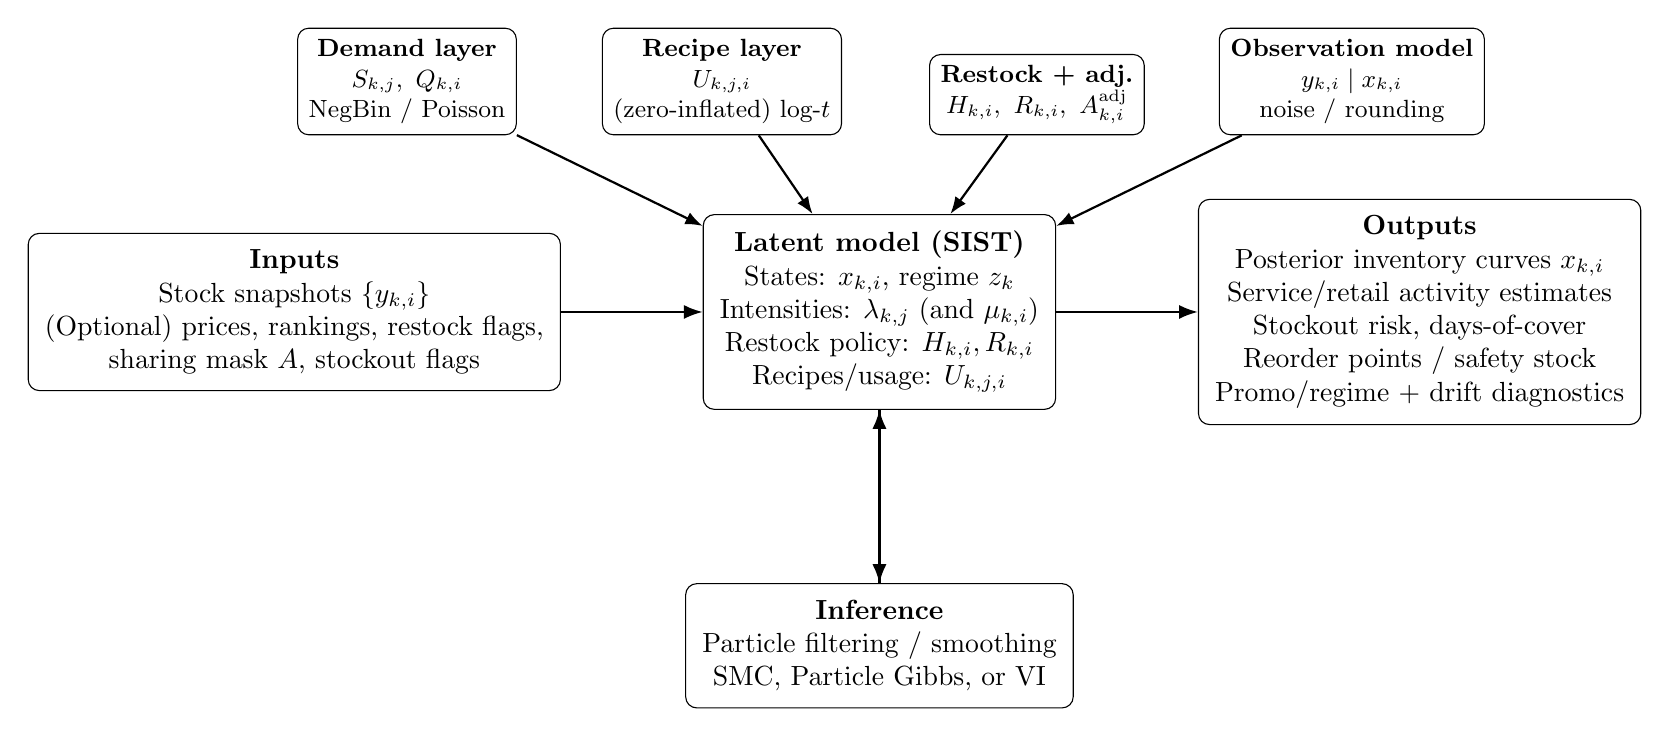
\begin{tikzpicture}[
  box/.style={draw, rounded corners, align=center, inner sep=6pt},
  subbox/.style={draw, rounded corners, align=center, inner sep=4pt, font=\small},
  arr/.style={-{Latex[length=2.4mm]}, thick},
  subarr/.style={-{Latex[length=2.2mm]}, thick}
]

\node[box] (inputs) {\textbf{Inputs}\\
Stock snapshots $\{y_{k,i}\}$\\
(Optional) prices, rankings, restock flags,\\sharing mask $A$, stockout flags};

\node[box, right=18mm of inputs] (model) {\textbf{Latent model (SIST)}\\
States: $x_{k,i}$, regime $z_k$\\
Intensities: $\lambda_{k,j}$ (and $\mu_{k,i}$)\\
Restock policy: $H_{k,i},R_{k,i}$\\
Recipes/usage: $U_{k,j,i}$};

\node[box, right=18mm of model] (outputs) {\textbf{Outputs}\\
Posterior inventory curves $x_{k,i}$\\
Service/retail activity estimates\\
Stockout risk, days-of-cover\\
Reorder points / safety stock\\
Promo/regime + drift diagnostics};

% Components that feed into SIST
\node[subbox, above=10mm of model, xshift=-60mm] (demand) {\textbf{Demand layer}\\
$S_{k,j},\ Q_{k,i}$\\
NegBin / Poisson};

\node[subbox, above=10mm of model, xshift=-20mm] (recipes) {\textbf{Recipe layer}\\
$U_{k,j,i}$\\
(zero-inflated) log-$t$};

\node[subbox, above=10mm of model, xshift=20mm] (restock) {\textbf{Restock + adj.}\\
$H_{k,i},\ R_{k,i},\ A^{\mathrm{adj}}_{k,i}$};

\node[subbox, above=10mm of model, xshift=60mm] (obs) {\textbf{Observation model}\\
$y_{k,i}\mid x_{k,i}$\\
noise / rounding};

\node[box, below=22mm of model] (inference) {\textbf{Inference}\\Particle filtering / smoothing\\SMC, Particle Gibbs, or VI};

\draw[arr] (inputs) -- (model);
\draw[arr] (model) -- (outputs);

\draw[subarr] (demand) -- (model);
\draw[subarr] (recipes) -- (model);
\draw[subarr] (restock) -- (model);
\draw[subarr] (obs) -- (model);

\draw[arr] (model) -- (inference);
\draw[arr] (inference) -- (model);

\end{tikzpicture}%
}%
\end{center}

Time is indexed by report times $t_1 < \dots < t_K$, with irregular gaps ($\Delta t_k = t_k - t_{k-1}$).

\textbf{Indices}
\begin{enumerate}
  \item SKU ($i \in \{1,\dots,I\}$)
  \item Service ($j \in \{1,\dots,J\}$)
  \item Bundle or promo service ($b \in \{1,\dots,B\}$) (optional explicit bundle types)
\end{enumerate}

\textbf{Definitions and notation}
\begin{enumerate}
  \item Report times: $t_1 < \dots < t_K$.
  \item Interval length: $\Delta t_k = t_k - t_{k-1}$.
  \item Inventory state: $x_{k,i}$ is on-hand inventory of SKU $i$ immediately after report $k$.
  \item Reported stock: $y_{k,i}$ is a noisy/rounded observation of $x_{k,i}$.
  \item Inventory update in interval $k$ for SKU $i$:
  \begin{enumerate}
    \item Let $D_{k,i}\ge 0$ denote \emph{latent (unconstrained) demand/usage} in the interval.
    \item Let $C_{k,i}$ denote \emph{realized} consumption/usage, capped by available inventory:
    \[
      C_{k,i} = \min\bigl\{D_{k,i},\ x_{k-1,i} + R_{k,i}\bigr\}.
    \]
    \item Let $A^{\mathrm{adj}}_{k,i}$ be a signed inventory correction (can be positive or negative).
    \item Then the inventory state update is
    \[
      x_{k,i} = \max\bigl\{0,\ x_{k-1,i} + R_{k,i} - C_{k,i} + A^{\mathrm{adj}}_{k,i}\bigr\}.
    \]
  \end{enumerate}
  Here $R_{k,i}\ge 0$ is total restock received over the interval.

  \item Services and retail:
  \begin{enumerate}
    \item $S_{k,j}$: count of service $j$ instances in interval $k$.
    \item $Q_{k,i}$: retail quantity of SKU $i$ in interval $k$ (if modeled).
  \end{enumerate}
  \item Regimes: $z_k$ is a discrete regime label controlling dispersion and/or recipe shifts.
  \begin{enumerate}
    \item \textbf{Normal:} baseline behavior; demand and recipes follow their usual drift/seasonal dynamics.

    \item \textbf{Spike:} short-lived demand surge (e.g., an event day). Typically increases mean intensity (larger $\lambda_{k,j}$ and/or $\mu_{k,i}$) and may increase dispersion (smaller $\kappa_{z_k,j}$ / $\phi_{z_k,i}$).

    \item \textbf{Lull:} unusually quiet interval. Typically decreases intensities and may also reduce dispersion (closer to Poisson-like behavior).

    \item \textbf{Stockout-constrained:} latent demand exists, but realized sales or usage are capped when inventory hits (or approaches) zero. In this regime, observed consumption is interpreted as \emph{censored} demand. The posterior favors trajectories with $\min_t x_i(t) \approx 0$ for at least one binding SKU.

    \item \textbf{Promo:} promotion period that shifts the service mix and/or usage recipes (e.g., different average inputs per service). Operationally this can mean shifted $\lambda_{k,j}$, different dispersions, and/or shifted recipe means $\mu^{\mathrm{use}}_{k,j,i}$.

    \item \textbf{Correction:} bookkeeping/measurement correction (late entry, recount, unit conversion, write-off). This regime increases the probability and/or scale of inventory corrections $A^{\mathrm{adj}}_{k,i}$ and can also inflate observation noise $\sigma_{\text{obs},i}$ for the affected interval.
  \end{enumerate}

  \item Distribution notation: $\text{Normal}^+(m,s^2)$ denotes a Normal$(m,s^2)$ truncated to $\mathbb{R}_{\ge 0}$.
\end{enumerate}

\textbf{Latent states and events per interval $k$}
\begin{enumerate}
  \item $x_{k,i}$: true on-hand inventory of SKU $i$ right after report $k$
  \item $z_k$: discrete regime (normal, spike, lull, stockout-constrained, promo, correction)
  \item $\lambda_{k,j}$: time-varying service intensity for service $j$
  \item $\mu_{k,i}$: time-varying retail intensity for SKU $i$ (optional)
  \item Restock policy parameters that can drift, for example $\alpha_{k,i}, \beta_{k,i}$
\end{enumerate}

\subsection*{Observed (required)}
\begin{enumerate}
  \item $y_{k,i}$: reported stock (noisy, possibly rounded)
\end{enumerate}

\subsection*{Observed (optional add-ons)}
\begin{enumerate}
  \item Prices (time-varying but infrequently updated):
  \begin{enumerate}
    \item $p^{\mathrm{svc}}_{k,j}$: price for service $j$ during interval $k$
    \item $p^{\mathrm{ret}}_{k,i}$: price for retail SKU $i$ during interval $k$
  \end{enumerate}

  \item Ranked lists per interval $k$ (no quantities):
  \begin{enumerate}
    \item $r^{\mathrm{svc}}_k$: ordering of top services in $\Delta t_k$
    \item $r^{\mathrm{ret}}_k$: ordering of top retail SKUs in $\Delta t_k$ (if retail is used)
  \end{enumerate}

  \item Restock-included flags per update (no quantities):
  \begin{enumerate}
    \item $\tilde{h}_{k,i} \in \{0,1\}$: user indicates whether the stock update includes a restock for SKU $i$ in $\Delta t_k$
  \end{enumerate}

  \item Service--SKU sharing mask (sparse recipe support):
  \begin{enumerate}
    \item $A_{j,i} \in \{0,1\}$: whether service $j$ can consume SKU $i$ (enables the connection)
    \item $\rho_{k,j,i} \in (0,1)$: probability that a given instance of service $j$ actually uses SKU $i$ in interval $k$ (optional)
  \end{enumerate}

  \item Stockout flags:
  \begin{enumerate}
    \item $o^{\mathrm{svc}}_{k,j} \in \{0,1\}$: whether service $j$ was unavailable at any point in $\Delta t_k$
    \item $o^{\mathrm{ret}}_{k,i} \in \{0,1\}$: whether retail SKU $i$ was unavailable at any point in $\Delta t_k$
  \end{enumerate}
\end{enumerate}

\section{Inventory dynamics}

For each SKU $i$, interval $k$:
\begin{enumerate}
  \item Let $D_{k,i}\ge 0$ denote latent (unconstrained) demand/usage in the interval.
  \item Let $C_{k,i}$ denote realized consumption/usage, capped by available inventory:
  \[
    C_{k,i} = \min\bigl\{D_{k,i},\ x_{k-1,i} + R_{k,i}\bigr\}.
  \]
  \item Inventory updates as
  \[
    x_{k,i} = \max\bigl\{0,\ x_{k-1,i} + R_{k,i} - C_{k,i} + A^{\mathrm{adj}}_{k,i}\bigr\}.
  \]
\end{enumerate}

We decompose latent demand into service and retail components:
\[
  D_{k,i} = C^{\mathrm{svc}}_{k,i} + C^{\mathrm{ret}}_{k,i}.
\]

Here $A^{\mathrm{adj}}_{k,i}$ is a signed correction term (e.g., recount, write-off, unit conversion).

\subsection{Services sold, latent counts}

Service counts are latent and regime dependent:
\[
  S_{k,j} \sim \text{NegBin}(\lambda_{k,j}\,\Delta t_k,\ \kappa_{z_k,j}).
\]

Negative Binomial is the default because it tolerates burstiness. Poisson is a special case.

\subsection{Stochastic recipes, real-valued usage}

Each service instance consumes a random amount of each SKU.

For one service $j$ and SKU $i$, per instance:
\[
  U_{k,j,i} \sim F_{k,j,i}.
\]

A strong default for positive real usage is a heavy-tailed log-Student-$t$ recipe:
\[
  \log U_{k,j,i} \sim \text{Student-}t_{\nu}\bigl(\mu^{\mathrm{use}}_{k,j,i},\ \sigma^{\mathrm{use}}_{j,i}\bigr).
\]

\textbf{Optional: zero-inflated (spike-and-slab) recipes.}

Setting $A_{j,i}=1$ means service $j$ \emph{can} consume SKU $i$, but it does not imply that SKU $i$ is used in \emph{every} instance of the service.
To capture ``sometimes uses SKU $i$, sometimes does not,'' introduce a per-instance usage indicator.

For each service instance $m=1,\dots,S_{k,j}$:
\[
  B^{(m)}_{k,j,i} \sim \text{Bernoulli}(\rho_{k,j,i}),\qquad B^{(m)}_{k,j,i} \in \{0,1\}.
\]
Then define
\[
  U^{(m)}_{k,j,i} = B^{(m)}_{k,j,i} \cdot \tilde U^{(m)}_{k,j,i},\qquad \tilde U^{(m)}_{k,j,i} > 0,
\]
with a positive recipe distribution for the slab, e.g.
\[
  \log \tilde U^{(m)}_{k,j,i} \sim \text{Student-}t_{\nu}\bigl(\mu^{\mathrm{use}}_{k,j,i},\ \sigma^{\mathrm{use}}_{j,i}\bigr).
\]
If $A_{j,i}=0$, enforce $B^{(m)}_{k,j,i}=0$ and hence $U^{(m)}_{k,j,i}=0$.

Total service consumption of SKU $i$ over the interval:
\[
  C^{\mathrm{svc}}_{k,i} = \sum_{j=1}^{J}\sum_{m=1}^{S_{k,j}} U^{(m)}_{k,j,i}.
\]

\subsection{Retail sales of SKUs}

If the user also sells SKUs as products, model retail quantity:
\[
  Q_{k,i} \sim \text{NegBin}(\mu_{k,i}\,\Delta t_k,\ \phi_{z_k,i}).
\]

Retail consumption contribution:
\[
  C^{\mathrm{ret}}_{k,i} = Q_{k,i} \cdot u^{\mathrm{ret}}_i,
\]

where $u^{\mathrm{ret}}_i$ is units per retail sale, often 1 or a known pack fraction.

\subsection{Adjustments and shrinkage}

Model adjustments as signed inventory corrections:
\[
  A^{\mathrm{adj}}_{k,i} \sim \text{Normal}\bigl(m^{\mathrm{adj}}_{z_k,i}\,\Delta t_k,\ (s^{\mathrm{adj}}_{z_k,i})^2\bigr).
\]

Interpretation:
\begin{enumerate}
  \item $A^{\mathrm{adj}}_{k,i}<0$ corresponds to shrinkage/write-offs (waste, spoilage, theft).
  \item $A^{\mathrm{adj}}_{k,i}>0$ corresponds to upward corrections (late entries, recounts, unit conversion fixes).
\end{enumerate}

Inventory is still clamped at zero in the update $x_{k,i}=\max\{0,\cdot\}$.

\subsection{Restocking as a policy}

Restocking is treated as a decision influenced by stock level and time.

\textbf{Restock event indicator.} Let $H_{k,i}\in\{0,1\}$ indicate whether SKU $i$ is restocked at least once during interval $k$.
We model $H_{k,i}$ as Bernoulli because many intervals have \emph{no} restock at all (a structural zero), and when restocks do occur they happen as discrete events:
\[
  H_{k,i} \sim \text{Bernoulli}(\pi_{k,i}).
\]

Here $\pi_{k,i}\in(0,1)$ is the restock probability in interval $k$ for SKU $i$.
To map a linear predictor to a valid probability we use the logistic link (logit), i.e.
$\text{logit}(p)=\log\!\bigl(p/(1-p)\bigr)$:
\[
  \text{logit}(\pi_{k,i}) = \alpha_{k,i} + \beta_{k,i} x_{k-1,i} + \gamma_i \cdot \text{age}_{k,i}.
\]

Interpretation of covariates/parameters:
\begin{enumerate}
  \item $x_{k-1,i}$ is the on-hand inventory right after report $k-1$ (lower inventory should generally increase restock propensity; this is typically captured by $\beta_{k,i}<0$).
  \item $\text{age}_{k,i}$ is time since last restock (or since last report if restocks are not observed), used to encode periodic ordering habits.
  \item $\alpha_{k,i}$ is a baseline log-odds of restocking for SKU $i$ in interval $k$.
  \item $\beta_{k,i}$ is sensitivity of restock propensity to current stock level.
  \item $\gamma_i$ is sensitivity to the elapsed time/age covariate.
\end{enumerate}

Given a restock happens, restock size is positive real:
\[
  R_{k,i} \sim
  \begin{cases}
    0 & \text{if } H_{k,i} = 0,\\
    \text{LogNormal}(\mu^{R}_{k,i},\ \sigma^{R}_i) & \text{if } H_{k,i} = 1.
  \end{cases}
\]

Here $\mu^{R}_{k,i}$ is the (log-scale) location parameter controlling the typical restock size for SKU $i$ in interval $k$, and $\sigma^{R}_i>0$ is the log-scale dispersion controlling how variable restock sizes are.
In practice, $\mu^{R}_{k,i}$ can be treated as time-varying (to reflect changing order quantities) while $\sigma^{R}_i$ is often approximately time-invariant.

This naturally captures sparse restocks with occasional large jumps.

\section{Promotions and bundles}

\textbf{Motivation.} Sparse inventory snapshots create an ill-posed inverse problem: many different latent demand paths can explain the same observed stock changes.
Promotions and bundles are two common real-world causes of structured, short-lived departures from baseline demand and usage.
Modeling them explicitly prevents the inference from incorrectly attributing promo-driven inventory drops to long-run drift, and improves identifiability by introducing interpretable structure (regime shifts and multi-SKU bundle signatures) that better matches how businesses actually operate.

SIST supports two mechanisms; both can be used together.

\subsection{Promotions as regimes}

Regime $z_k$ changes service mix, prices, and recipe parameters.

In the \textbf{promo} regime, the model allows systematic departures from baseline behavior, for example:
\begin{enumerate}
  \item \textbf{Demand lift and mix shift:} services may become more (or less) frequent, so the service intensities $\lambda_{k,j}$ can shift relative to non-promo periods. Importantly, the \emph{composition} of demand across services can change, not just the total volume.

  \item \textbf{Recipe/usage shift:} promotions can change how SKUs are consumed per service (e.g., different bundle contents, portion sizes, substitutions, or free add-ons). This is captured by allowing recipe parameters---especially the recipe means $\mu^{\mathrm{use}}_{k,j,i}$ (and optionally dispersions $\sigma^{\mathrm{use}}_{j,i}$)---to shift under promo.

  \item \textbf{Dispersion changes:} promos can increase burstiness and heterogeneity across days, which can be modeled via regime-specific overdispersion (e.g., smaller $\kappa_{z_k,j}$ for service counts, and smaller $\phi_{z_k,i}$ for retail counts if retail is modeled).

  \item \textbf{Price and bundle effects (if observed):} if prices $p^{\mathrm{svc}}_{k,j}$ / $p^{\mathrm{ret}}_{k,i}$ or bundle indicators are provided, promo periods can be tied to those changes to improve identifiability of whether inventory drops are driven by higher demand, changed recipes, or both.
\end{enumerate}

Operationally, the promo regime is a structured way to let a small number of intervals ``break the rules'' of smooth drift/seasonality while still pooling information across time.

\subsection{Promotion-bundles as explicit services}

A common failure mode with sparse inventory reports is \emph{non-identifiability}: many different combinations of services could explain the same net SKU drawdown.
Explicit bundles reduce this ambiguity.

Introduce a set of bundle (or promo) service types indexed by $b\in\{1,\dots,B\}$.
Each bundle $b$ is treated as a service with its own latent count $S_{k,b}$, price $p^{\mathrm{svc}}_{k,b}$ (if prices are tracked), and recipe distribution over SKUs $F_{k,b,i}$:
\begin{enumerate}
  \item \textbf{Bundle counts:} infer $S_{k,b}$ in the same way as any service count (e.g., via a Negative Binomial intensity model). This lets the model explain bursts of joint multi-SKU consumption by attributing them to bundle sales.

  \item \textbf{Bundle recipes:} bundles often consume a \emph{structured set} of SKUs (e.g., ``cut + style + shampoo'' or ``service + take-home product''). These multi-SKU signatures make it easier to distinguish bundle-driven consumption from coincidental co-movement across independent services.

  \item \textbf{Identifiability gain:} when inventory drops across several SKUs occur together, the posterior can put mass on bundle events instead of forcing implausible correlated spikes across many base services.

  \item \textbf{Interpretability:} the inferred $S_{k,b}$ provides a direct estimate of promo uptake (with uncertainty), which is often more actionable than changes in individual $\lambda_{k,j}$ alone.
\end{enumerate}

In short, explicit bundles add a small number of structured latent variables that can explain joint SKU movements, improving both inference stability and business interpretability.

\section{Drift handling: gradual, seasonal, abrupt}

\textbf{Motivation.} Real businesses rarely have stationary demand or stationary ``recipes'' for SKU usage: staff behavior changes, product lines evolve, prices and competitors move, and there are seasonal patterns.
If SIST assumed fixed intensities and fixed usage parameters, it would systematically misattribute slow changes to noise and would overfit old history.
Drift dynamics provide controlled forgetting: they let the posterior adapt to new behavior while still borrowing strength from past observations.

SIST includes three complementary types of drift:
\begin{enumerate}
  \item \textbf{Gradual drift:} smooth, persistent evolution in demand rates and/or recipes, modeled as time-varying latent states (e.g., random-walk dynamics on $\log \lambda_{k,j}$ and optionally on recipe means $\mu^{\mathrm{use}}_{k,j,i}$).
  \item \textbf{Seasonal drift:} predictable periodic patterns (day-of-week, month-of-year), modeled as additive covariates (e.g., $w_{j,\text{dow}}$ and $w_{j,\text{month}}$) with shrinkage so they only activate when supported by data.
  \item \textbf{Abrupt drift:} rare structural breaks (new menu, supplier change, policy change, accounting correction), modeled via change points $c_k$ that allow partial resets or jumps in intensities and/or recipe parameters.
\end{enumerate}

\subsection{Gradual drift via time-varying intensities}

\textbf{What drifts.} The main quantities that evolve over time are service intensities $\lambda_{k,j}$ (expected service activity per unit time) and, optionally, recipe means $\mu^{\mathrm{use}}_{k,j,i}$ (typical log-usage of SKU $i$ per instance of service $j$).

\textbf{Why drift on the log scale.} Intensities must stay positive ($\lambda_{k,j}>0$), so we model a random walk on $\log \lambda_{k,j}$.
This turns multiplicative changes (e.g., ``demand is up 20\%'') into approximately additive increments.

Service intensities drift:
\[
  \log \lambda_{k,j} = \log \lambda_{k-1,j} + \epsilon_{k,j},
\]
\[
  \epsilon_{k,j} \sim \text{Student-}t_{\nu_{\lambda}}\bigl(0,\ \sigma_{\lambda,j}\bigr).
\]

Definitions:
\begin{enumerate}
  \item $\epsilon_{k,j}$ is the increment (shock) to the log-intensity for service $j$ in interval $k$.
  \item $\nu_{\lambda}$ is the degrees-of-freedom controlling tail-heaviness; smaller values allow occasional larger jumps.
  \item $\sigma_{\lambda,j}>0$ is the drift scale for service $j$; larger values mean faster-changing demand.
\end{enumerate}

Retail intensities drift similarly if used (replace $\lambda_{k,j}$ with $\mu_{k,i}$).

Recipe mean drift (optional):
\[
  \mu^{\mathrm{use}}_{k,j,i} = \mu^{\mathrm{use}}_{k-1,j,i} + \eta_{k,j,i},
\]
\[
  \eta_{k,j,i} \sim \text{Normal}(0,\ \sigma^2_{\mu,j,i}).
\]

Here $\eta_{k,j,i}$ is the per-interval recipe-mean increment and $\sigma_{\mu,j,i}>0$ controls how quickly usage norms change.

\subsection{Seasonality as covariates with shrinkage}

Seasonality captures repeatable patterns (e.g., weekends) that are not well represented by a random walk.
For each service $j$, add calendar effects to the log-intensity:
\[
  \log \lambda_{k,j} \mathrel{+}= w_{j,\text{dow}}(\text{day of week}) + w_{j,\text{month}}(\text{month}).
\]

Here $w_{j,\text{dow}}(d)$ is the day-of-week effect (a 7-vector per service) and $w_{j,\text{month}}(m)$ is the month-of-year effect (a 12-vector per service).

\textbf{What ``shrinkage priors'' means.} A \emph{prior} is a probability distribution placed on an unknown parameter before seeing the current user's data.
A \emph{shrinkage prior} is a prior centered at 0 with most of its mass near 0, so that in the absence of strong evidence the posterior prefers small seasonal effects (i.e., $w\approx 0$).
This prevents overfitting when the time series is short or sparse.

A simple shrinkage choice is, for each service $j$,
\[
  w_{j,\text{dow}}(d) \sim \text{Normal}(0,\ \sigma^2_{\text{dow},j}),\qquad
  w_{j,\text{month}}(m) \sim \text{Normal}(0,\ \sigma^2_{\text{month},j}),
\]
with small scales $\sigma_{\text{dow},j},\sigma_{\text{month},j}$ (see Section~\ref{sec:hyperparams} for a hierarchical default).

\textbf{How $w$ is estimated.} During inference, these priors combine with the likelihood implied by the observed stock reports (and any optional signals) to produce a posterior over $w$.
If the data repeatedly show higher inferred demand on (say) weekends for service $j$, the posterior for the corresponding components of $w_{j,\text{dow}}$ moves away from 0; otherwise it stays near 0.

\subsection{Abrupt drift via occasional change points}

Abrupt drift handles rare structural breaks (new menu, staff changes, supplier changes).
We introduce a change-point indicator:
\[
  c_k \sim \text{Bernoulli}(p_c),
\]

where $p_c\in(0,1)$ is the per-interval change-point probability.
If $c_k = 1$, the model allows a partial reset or jump in intensities and/or recipe parameters toward their priors (or toward a new regime-specific baseline).
If $c_k = 0$, parameters continue under the gradual drift/seasonal dynamics.

\section{Observation model for sparse stock reports}

Inventory is only observed intermittently, and reported values may be rounded or measured with error.
We model the reported stock as a noisy observation of the latent true on-hand inventory.

\textbf{Variables.}
\begin{enumerate}
  \item $x_{k,i}$ is the latent on-hand inventory of SKU $i$ immediately after report $k$.
  \item $y_{k,i}$ is the reported/measured stock value for SKU $i$ at report $k$.
  \item $\sigma_{\text{obs},i}>0$ is an SKU-specific observation-noise scale capturing counting error, scale/rounding noise, and minor reporting inconsistencies.
\end{enumerate}

\textbf{Gaussian observation model.} A simple default is:
\[
  y_{k,i} \sim \text{Normal}(x_{k,i},\ \sigma^2_{\text{obs},i}).
\]

\textbf{Rounding (optional).} If users tend to report in coarse increments (e.g., ``about 10''), treat $y_{k,i}$ as a rounded version of an underlying noisy measurement, e.g., by adding an explicit rounding operator or a mixture model that puts extra mass on common multiples.

\subsubsection*{Optional minimal user inputs as extra observations}

These inputs are designed to be low-effort (binary/categorical/ordinal) while materially improving identifiability.

\textbf{(i) Ranked lists of services / SKUs}

Users often know \emph{which} services/SKUs were most common in an interval, even if they do not know the exact counts.
SIST can use this information as an \emph{ordinal} observation that constrains the latent intensities.

\textbf{What the user provides.}
\begin{enumerate}
  \item $r^{\mathrm{svc}}_k$ is an ordering of the top services during interval $k$ (e.g., $[j_1 \succ j_2 \succ j_3]$).
  \item Optionally, $r^{\mathrm{ret}}_k$ is an ordering of the top retail SKUs during interval $k$.
\end{enumerate}

\textbf{What it means in the model.} If service $a$ is ranked above $b$ (denoted $a\succ b$), we interpret it as evidence that the activity rate for $a$ exceeded that of $b$ during interval $k$.
A simple (pairwise) likelihood is:
\[
  P(a \succ b \mid \lambda_{k,*}) = \sigma\!\left(\frac{\log \lambda_{k,a} - \log \lambda_{k,b}}{\tau}\right),
\]

where $\sigma(u)=1/(1+e^{-u})$ is the logistic function and $\tau>0$ is a \emph{temperature} controlling ranking noise.
As $\tau\to 0$, the ranking becomes nearly deterministic; larger $\tau$ makes rankings less informative.

\textbf{How a top-$N$ list becomes constraints.} If the list is $[j_1 \succ j_2 \succ \dots \succ j_N]$, add pairwise comparisons for all adjacent pairs $j_1\succ j_2$, $j_2\succ j_3$, \dots, $j_{N-1}\succ j_N$ (or, more strongly, for all pairs $j_a\succ j_b$ with $a<b$).
Items not listed are treated as ``unranked'' (no constraint) unless the user explicitly asserts they were below the top-$N$.

\textbf{Notes.} If ties are common, treat them as weak constraints (e.g., skip tied pairs or use a wide-$\tau$ likelihood).
More structured ranking likelihoods (e.g., Plackett--Luce) can be substituted, but the pairwise form is a robust default.

\textbf{(ii) Restock-included flags}

A common ambiguity with sparse stock snapshots is whether a jump in reported inventory was caused by \emph{restocking} or by \emph{reduced consumption}.
A low-effort way to disambiguate is to let the user mark which updates include a restock.

\textbf{What the user provides.} $\tilde{h}_{k,i}\in\{0,1\}$ indicates whether the report-to-report change for SKU $i$ over interval $\Delta t_k$ included a restock event.
This is an \emph{indicator only} (no quantity).

\textbf{How it enters the model.} Recall the latent restock-event indicator $H_{k,i}\in\{0,1\}$ from the restock policy.
Treat $\tilde{h}_{k,i}$ as a noisy observation of $H_{k,i}$ (rather than a hard constraint), for example:
\[
  P(\tilde{h}_{k,i}=1\mid H_{k,i}=1)=\pi^{\mathrm{TP}}_i,\qquad
  P(\tilde{h}_{k,i}=1\mid H_{k,i}=0)=\pi^{\mathrm{FP}}_i,
\]
with $\pi^{\mathrm{TP}}_i$ near 1 and $\pi^{\mathrm{FP}}_i$ near 0.

This keeps the restock policy interpretable while still leveraging the user-provided flag.

\textbf{(iii) Service--SKU sharing mask}

Another major source of non-identifiability is unknown recipe support: without constraints, any service can (in principle) consume any SKU.
A sparse support mask makes the inference more realistic and stable.

\textbf{What the user provides.} $A_{j,i}\in\{0,1\}$ indicates whether service $j$ can consume SKU $i$ at all (e.g., shampoo is used by ``wash'' services, but not by ``consultation'').
In practice this can come from a point-of-sale menu, a bill-of-materials template, or a simple checkbox UI.

\textbf{How it enters the model.} For latent per-instance usage $U_{k,j,i}$:
\begin{enumerate}
  \item If $A_{j,i}=0$, enforce $U_{k,j,i}=0$ for all $k$ (structural zero).
  \item If $A_{j,i}=1$, draw usage from the recipe distribution $F_{k,j,i}$.
\end{enumerate}

This focuses posterior mass on plausible explanations and reduces spurious cross-SKU attribution.

\textbf{(iv) Stockout flags}

Stockouts turn observed sales into \emph{censored} demand: low observed consumption may reflect lack of inventory, not lack of customers.
Stockout flags help the model distinguish these cases.

\textbf{What the user provides.}
\begin{enumerate}
  \item $o^{\mathrm{svc}}_{k,j}\in\{0,1\}$ indicates whether service $j$ was unavailable at any point during $\Delta t_k$.
  \item $o^{\mathrm{ret}}_{k,i}\in\{0,1\}$ indicates whether retail SKU $i$ was unavailable at any point during $\Delta t_k$.
\end{enumerate}

\textbf{How it enters the model.}
\begin{enumerate}
  \item If $o^{\mathrm{svc}}_{k,j}=1$, upweight trajectories where at least one required SKU (with $A_{j,i}=1$) hits (or closely approaches) zero during $\Delta t_k$, implying demand was partially blocked.
  \item If $o^{\mathrm{svc}}_{k,j}=0$, downweight trajectories that would force service $j$ to be stockout-constrained.

  \item If $o^{\mathrm{ret}}_{k,i}=1$, upweight trajectories where SKU $i$ hits (or closely approaches) zero during $\Delta t_k$.
  \item If $o^{\mathrm{ret}}_{k,i}=0$, downweight trajectories that would require SKU $i$ to be at (or near) zero for extended periods.
\end{enumerate}

In effect, the flags provide a qualitative observation about within-interval availability that is otherwise unidentifiable from sparse snapshot data.

\subsubsection*{Hyperparameters and default priors}\label{sec:hyperparams}

This section lists suggested weakly-informative default priors for key hyperparameters.
Where possible, predictors should be scaled so that typical values are $O(1)$.

\textbf{Negative Binomial parameterization}

Assume $\text{NegBin}(m,\kappa)$ is parameterized by mean $m>0$ and dispersion $\kappa>0$:
\[
  E[Y]=m,\qquad \mathrm{Var}(Y)=m + \frac{m^2}{\kappa}.
\]
Then larger $\kappa$ is closer to Poisson.
(Equivalently, if you use a $(r,p)$ parameterization with $Y\sim\text{NegBin}(r,p)$ and support $Y\in\{0,1,2,\dots\}$, set
$r=\kappa$ and $p=\kappa/(\kappa+m)$ so that $E[Y]=m$.)

\textbf{Count dispersion}
\begin{enumerate}
  \item Service overdispersion: $\kappa_{z_k,j} > 0$.
  \item Retail overdispersion: $\phi_{z_k,i} > 0$.
\end{enumerate}
Default: initialize $\kappa_{z_k,j}$ and $\phi_{z_k,i}$ at $1$ (moderate overdispersion) as starting values for inference/optimization.
Priors: $\kappa_{z_k,j} \sim \text{Exponential}(1)$ and $\phi_{z_k,i} \sim \text{Exponential}(1)$.

\textbf{Recipe noise and drift scales}
\begin{enumerate}
  \item Recipe log-scale noise: $\sigma^{\mathrm{use}}_{j,i} > 0$.
  \item Intensity drift scale: $\sigma_{\lambda,j} > 0$.
  \item Recipe mean drift scale: $\sigma_{\mu,j,i} > 0$ (via $\eta_{k,j,i}\sim\text{Normal}(0,\sigma^2_{\mu,j,i})$).
\end{enumerate}
Defaults: initialize $\sigma^{\mathrm{use}}_{j,i}$, $\sigma_{\lambda,j}$, and $\sigma_{\mu,j,i}$ at small values after standardizing units (e.g., $0.1$--$0.5$ on a log scale).
(Here $\sigma^{\mathrm{use}}_{j,i}$ appears in $\log U_{k,j,i}$, $\sigma_{\lambda,j}$ appears in the drift increment $\epsilon_{k,j}$ for $\log\lambda_{k,j}$, and $\sigma_{\mu,j,i}$ appears in the recipe-mean drift increment $\eta_{k,j,i}$.)
Priors (weakly-informative):
\[
  \sigma^{\mathrm{use}}_{j,i},\ \sigma_{\lambda,j},\ \sigma_{\mu,j,i} \sim \text{Half-}t_{4}(0,\ s),
\]
with a global scale $s>0$.
Default: set $s=1$ after scaling so that typical log-variations are $O(1)$.

\textbf{Zero-inflation probability (optional)}

If using the spike-and-slab recipe layer, $\rho_{k,j,i} \in (0,1)$ controls how often SKU $i$ is used when $A_{j,i}=1$.
A simple default is a weak prior:
\[
  \rho_{k,j,i} \sim \text{Beta}(1,1).
\]
Optionally, $\text{logit}(\rho_{k,j,i})$ can be given a drift model analogous to $\log \lambda_{k,j}$.

\textbf{Seasonality shrinkage (hierarchical).}
\[
  w_{j,\text{dow}}(d) \sim \text{Normal}(0,\ \sigma^2_{\text{dow},j}),\qquad
  w_{j,\text{month}}(m) \sim \text{Normal}(0,\ \sigma^2_{\text{month},j}).
\]
\[
  \sigma_{\text{dow},j} \sim \text{HalfNormal}(0,\ \tau_{\text{dow}}),\qquad
  \sigma_{\text{month},j} \sim \text{HalfNormal}(0,\ \tau_{\text{month}}).
\]
\[
  \tau_{\text{dow}} \sim \text{HalfNormal}(0,\ 1),\qquad
  \tau_{\text{month}} \sim \text{HalfNormal}(0,\ 1).
\]
Defaults: initialize $\tau_{\text{dow}}=0.3$ and $\tau_{\text{month}}=0.3$.
(Here $\tau_{\text{dow}}$ and $\tau_{\text{month}}$ are global hyperparameters controlling the typical magnitude of day-of-week and month effects across services; smaller values imply stronger shrinkage toward $w\approx 0$.)

\textbf{Observation noise}

Observation noise per SKU: $\sigma_{\text{obs},i} > 0$.
This parameter appears in the observation model
$y_{k,i}\sim\text{Normal}(x_{k,i},\sigma^2_{\text{obs},i})$ and summarizes counting error plus any effective noise induced by rounding.

Default: initialize $\sigma_{\text{obs},i}$ to the typical reporting resolution for SKU $i$ (e.g., if counts are usually within $\pm 1$, start at $1$; if reports are in steps of 5, start at $2$--$5$).
Prior: $\sigma_{\text{obs},i} \sim \text{HalfNormal}(0,\ s_{\text{obs}})$.
Default: set $s_{\text{obs}}=5$ in raw ``units'' (or $s_{\text{obs}}=1$ after scaling each SKU to unit variance).

\textbf{Adjustment model}

Recall the signed inventory-correction component
$A^{\mathrm{adj}}_{k,i} \sim \text{Normal}\bigl(m^{\mathrm{adj}}_{z_k,i}\,\Delta t_k,(s^{\mathrm{adj}}_{z_k,i})^2\bigr)$.
Here $s^{\mathrm{adj}}_{z_k,i}>0$ is the correction noise (in SKU units) for SKU $i$ under regime $z_k$.

Default: initialize $s^{\mathrm{adj}}_{z_k,i}=1$ after scaling (or to a small number of physical units if unscaled).
Prior: $s^{\mathrm{adj}}_{z_k,i} \sim \text{Half-}t_{4}(0,\ s_{\text{adj}})$.
Default: set $s_{\text{adj}}=1$ after scaling.

\textbf{Restock policy coefficients}

These coefficients appear in the restock-propensity model
$\text{logit}(\pi_{k,i}) = \alpha_{k,i} + \beta_{k,i}x_{k-1,i} + \gamma_i\,\text{age}_{k,i}$.
For scaled predictors, use robust priors:
\[
  \alpha_{k,i},\ \beta_{k,i},\ \gamma_i \sim \text{Student-}t_{3}(0,\ 2.5).
\]

Interpretation: $\alpha_{k,i}$ is a baseline log-odds; $\beta_{k,i}$ controls sensitivity to stock level (often negative); $\gamma_i$ controls sensitivity to age/time-since-restock.
The scale 2.5 is on the log-odds scale (a typical weakly-informative logistic-regression default).

\textbf{Restock size model}

Restock size noise: $\sigma^{R}_i > 0$.
This parameter appears in the LogNormal restock-size model
$R_{k,i}\mid(H_{k,i}=1)\sim\text{LogNormal}(\mu^R_{k,i},\sigma^R_i)$ and controls multiplicative variability in order sizes.

Default: initialize $\sigma^{R}_i=0.3$ (on the log scale) after scaling; smaller values imply more consistent order sizes.
Prior: $\sigma^{R}_i \sim \text{Half-}t_{4}(0,\ s_R)$.
Default: set $s_R=1$ after scaling.

\textbf{Change-point probability}

$p_c \in (0,1)$ is the per-interval change-point probability in
$c_k\sim\text{Bernoulli}(p_c)$.

Default: small (e.g. $0.01$ per interval), corresponding to an expected change-point spacing of about $1/p_c=100$ intervals.
Prior: $p_c \sim \text{Beta}(1,1)$.

\textbf{Price update hyperparameters}

For each service $j$ and retail SKU $i$ (or globally, if you prefer):
\begin{enumerate}
  \item Price update probability: $p^{\mathrm{price}} \in (0,1)$.
  This is the per-interval probability that a posted price changes (i.e., the Bernoulli rate in $g^{\mathrm{svc}}_{k,j}\sim\text{Bernoulli}(p^{\mathrm{price}})$ and similarly for retail).
  Default: small (e.g. $0.01$ per interval).
  Prior: $p^{\mathrm{price}} \sim \text{Beta}(1,1)$.

  \item Price jump scale: $\sigma^{\mathrm{price}} > 0$.
  Interpreted on the log-multiplier scale (i.e., if a change occurs, $p\leftarrow p\exp(\xi)$ with $\xi\sim\text{Normal}(0,(\sigma^{\mathrm{price}})^2)$).
  Default: small (e.g. $0.05$).
  Prior: $\sigma^{\mathrm{price}} \sim \text{HalfNormal}(0,1)$.
\end{enumerate}

\textbf{Student-$t$ degrees of freedom}

This degrees-of-freedom parameter controls tail-heaviness for Student-$t$ components.
In SIST it appears in (at least) two places:
\begin{enumerate}
  \item Recipe noise (log-usage): $\log U_{k,j,i}\sim\text{Student-}t_{\nu}(\cdot)$.
  \item Drift shocks: $\epsilon_{k,j}\sim\text{Student-}t_{\nu_{\lambda}}(0,\sigma_{\lambda,j})$.
\end{enumerate}

For heavy tails with finite variance, a practical default is $\nu=4$ (and similarly $\nu_{\lambda}=4$).
If inferred, use a proper prior; a simple discrete option is:
\[
  \nu \in \{4,7,10,20,30\},\qquad P(\nu=4)\text{ largest.}
\]
Similarly for $\nu_{\lambda}$.

\textbf{Ranking temperature}

Temperature for the ordinal (ranking) likelihood: $\tau>0$.
This is the parameter in
$P(a\succ b\mid\lambda)=\sigma\bigl((\log\lambda_{k,a}-\log\lambda_{k,b})/\tau\bigr)$.
(It is unrelated to the seasonality hyperparameters $\tau_{\text{dow}}$ and $\tau_{\text{month}}$.)

Default: $\tau=1$.
Prior: $\tau \sim \text{HalfNormal}(0,1)$.
Equivalently, $\log \tau \sim \text{Normal}(0,1)$.

Optionally add rounding, for example a mixture that snaps to common increments.

Optional reporting timing model (only if you want to leverage the fact that users tend to report when stock is low):
\[
  P(\text{report at } t \mid x(t)) \propto \text{sigmoid}(a + b\,x(t) + d\,\text{age}).
\]

This can reduce bias when reports are not random.

\section{Revenue and cost as posterior-derived quantities}\label{sec:revenue}

Given prices $p^{\mathrm{svc}}_{k,j}$, $p^{\mathrm{ret}}_{k,i}$ and costs $c_i$:

\subsection*{Price dynamics (optional)}

Prices can change over time but typically only at a few update points.
Model each price series as piecewise constant with infrequent jumps.

For services (analogous for retail), let $g^{\mathrm{svc}}_{k,j} \in \{0,1\}$ indicate a price update event:
\[
  g^{\mathrm{svc}}_{k,j} \sim \text{Bernoulli}(p^{\mathrm{price}}).
\]
If $g^{\mathrm{svc}}_{k,j}=0$, keep the previous price; if $g^{\mathrm{svc}}_{k,j}=1$, draw a new price:
\[
  p^{\mathrm{svc}}_{k,j} =
  \begin{cases}
    p^{\mathrm{svc}}_{k-1,j} & \text{if } g^{\mathrm{svc}}_{k,j}=0,\\
    p^{\mathrm{svc}}_{k-1,j}\,\exp(\xi^{\mathrm{svc}}_{k,j}) & \text{if } g^{\mathrm{svc}}_{k,j}=1,
  \end{cases}
\]
\[
  \xi^{\mathrm{svc}}_{k,j} \sim \text{Normal}(0,\ (\sigma^{\mathrm{price}}_{j})^2).
\]

In applications where the user supplies the posted prices, treat $p^{\mathrm{svc}}_{k,j}$ and $p^{\mathrm{ret}}_{k,i}$ as observed; otherwise this provides a prior that allows rare updates.

Revenue in interval:
\[
  \text{Rev}_k = \sum_j p^{\mathrm{svc}}_{k,j} S_{k,j} + \sum_i p^{\mathrm{ret}}_{k,i} Q_{k,i}.
\]

Cost of restocking:
\[
  \text{Cost}^{\mathrm{restock}}_k = \sum_i c_i R_{k,i}.
\]

Cost of goods used:
\[
  \text{COGS}^{\mathrm{used}}_k = \sum_i c_i C_{k,i}.
\]

Because the system is Bayesian, each of these is a distribution, not a single number.

\section{What SIST outputs for one user}

All outputs below are posterior summaries computed from draws of latent trajectories
and model parameters.

\begin{enumerate}
  \item \textbf{Probabilistic inventory state (per SKU $i$)}
  \begin{enumerate}
    \item Posterior at each report: $p(x_{k,i}\mid\text{data})$ (mean, median, and credible intervals).
    \item Probability of being at/near zero: $P(x_{k,i}=0\mid\text{data})$ or $P(x_{k,i}\le \epsilon\mid\text{data})$.
    \item Change decomposition by interval $k$ (latent drivers):
    $\Delta x_{k,i} = R_{k,i} - D_{k,i} + A^{\mathrm{adj}}_{k,i}$,
    where $D_{k,i}=C^{\mathrm{svc}}_{k,i}+C^{\mathrm{ret}}_{k,i}$ is latent (unconstrained) demand.
  \end{enumerate}

  \item \textbf{Demand and activity inference}
  \begin{enumerate}
    \item Service counts and intensities: posterior for $S_{k,j}$ and $\lambda_{k,j}$.
    \item Retail quantities and intensities (if used): posterior for $Q_{k,i}$ and $\mu_{k,i}$.
    \item SKU driver attribution: e.g.
    $P\bigl(C^{\mathrm{svc}}_{k,i} > C^{\mathrm{ret}}_{k,i}\mid\text{data}\bigr)$.
  \end{enumerate}

  \item \textbf{Demand-rate features for planning (per SKU)}

  Define the latent per-time demand rate in interval $k$:
  \[
    d_{k,i} \equiv \frac{D_{k,i}}{\Delta t_k}.
  \]

  SIST outputs (optionally regime-conditional by $z_k$):
  \begin{enumerate}
    \item $E[d_{k,i}\mid\text{data}]$ and credible intervals for $d_{k,i}$.
    \item Short-horizon forecast distribution for demand rate $d_{k+1,i}$ from drift/seasonality dynamics.
  \end{enumerate}

  \item \textbf{Stockout risk and days-of-cover}
  \begin{enumerate}
    \item Interval stockout probability (approximated via simulated within-interval trajectories):
    \[
      \text{SOR}_{k,i} \equiv P\Bigl(\min_{t\in[t_{k-1},t_k]} x_i(t)=0\ \Big|\ \text{data}\Bigr).
    \]
    \item Days of cover at report $k$:
    \[
      \text{DoC}_{k,i} \equiv \frac{x_{k,i}}{\hat d_{k,i}},
    \]
    where $\hat d_{k,i}$ is a chosen posterior summary of the \emph{latent} demand rate $d_{k,i}$ (mean or a conservative quantile).
  \end{enumerate}

  \item \textbf{Lead time estimation (per SKU)}

  Let $L_i$ denote procurement lead time (days). If the user supplies a typical lead time,
  use it as a prior anchor; otherwise infer from historical restock timing when identifiable.

  A simple Bayesian lead-time model is:
  \[
    L_i \sim \text{LogNormal}(\mu^{L}_i,\ \sigma^{L}_i).
  \]

  SIST outputs $p(L_i\mid\text{data})$ and summaries such as $E[L_i\mid\text{data}]$ and $\mathrm{sd}(L_i\mid\text{data})$.

  \item \textbf{Safety stock, reorder point, and reorder triggers}

  Fix a target cycle service level $\beta$ (e.g., $0.95$) and let $z_{\beta}$ be the corresponding Normal quantile.

  Using the posterior for demand rate and lead time, approximate demand during lead time as
  $D^{\mathrm{LT}}_i \approx d_i\,L_i$.

  A convenient approximation that accounts for both demand and lead-time uncertainty is:
  \[
    \text{SS}_i \approx z_{\beta}\,\sqrt{E[L_i]\,\mathrm{Var}(d_i) + (E[d_i])^2\,\mathrm{Var}(L_i)},
  \]
  with expectations/variances taken under the current posterior (optionally conditioned on $z_k$).

  Expected demand during lead time:
  \[
    E[D^{\mathrm{LT}}_i] \approx E[d_i]\,E[L_i].
  \]

  Reorder point:
  \[
    \text{ROP}_i \equiv E[D^{\mathrm{LT}}_i] + \text{SS}_i.
  \]

  A fully Bayesian alternative (recommended) is to set:
  \[
    \text{ROP}_i = Q_{\beta}\bigl(D^{\mathrm{LT}}_i\bigr),
  \]
  where $Q_{\beta}$ is the posterior quantile computed directly from draws of $d_i$ and $L_i$.

  Reorder trigger probability at report $k$:
  \[
    P\bigl(x_{k,i} \le \text{ROP}_i\mid\text{data}\bigr).
  \]

  \item \textbf{Promo/regime diagnostics and drift alerts}
  \begin{enumerate}
    \item Posterior over regimes $p(z_k\mid\text{data})$ and regime-conditioned demand summaries.
    \item Change-point probabilities (if enabled) and drift magnitude indicators.
  \end{enumerate}

  \item \textbf{Profit proxy distributions}

  Posterior distributions for revenue, restock cost, and COGS (Section~\ref{sec:revenue}), plus optional regime-conditional profit proxies.
\end{enumerate}

\section{Evaluation protocol for publication readiness}

For publication, SIST should be evaluated as an inferential system and as a decision-support system. The following protocol makes claims falsifiable and comparable.

\begin{enumerate}
  \item \textbf{Synthetic recovery study.} Simulate data from known parameters and report recovery quality for key latent quantities ($x_{k,i}$, $S_{k,j}$, $R_{k,i}$, $z_k$), including credible-interval coverage and calibration.

  \item \textbf{Posterior predictive checks.} Compare replicated data to observed summaries that matter operationally: snapshot deltas, near-zero frequencies, top-ranked services/SKUs, and restock-event rates.

  \item \textbf{Forecasting benchmarks.} On rolling holdouts, compare demand-rate and stockout-risk forecasts against simpler baselines (e.g., intermittent-demand heuristics and non-drift variants), reporting proper scoring rules and coverage.

  \item \textbf{Decision-quality backtest.} Evaluate reorder performance under posterior-driven triggers versus baseline rules, using fill rate, realized stockout fraction, average on-hand inventory, and reorder frequency.

  \item \textbf{Ablation of optional signals.} Quantify the marginal value of each optional signal family (rankings, restock flags, sharing mask, stockout flags, prices) on calibration and downstream decisions.

  \item \textbf{Robustness and sensitivity.} Stress-test prior scales, $p_c$, and observation-noise assumptions; report which outputs remain stable.
\end{enumerate}

This evaluation plan is intentionally aligned with deployment goals: uncertainty calibration, forecast reliability, and improved replenishment decisions.

\section{Limitations}

\begin{enumerate}
  \item \textbf{Discrete units / pack sizes.} The default recipe layer models per-instance usage as positive real-valued and heavy-tailed (e.g., log-Student-$t$). For SKUs that are inherently discrete (bottles, packets) or sold in fixed pack sizes, a quantized/rounded usage model may be more appropriate.

  \item \textbf{Within-interval timing is collapsed.} SIST models net effects over each reporting interval $\Delta t_k$. If restocks and consumption interleave within an interval, the exact stockout timing and lost-sales duration can be weakly identified without finer-grained data.

  \item \textbf{Censoring is stylized.} The cap $C_{k,i}=\min\{D_{k,i},x_{k-1,i}+R_{k,i}\}$ enforces feasibility at the interval level, but it is still an approximation to true censoring/lost-sales processes that depend on the path $x_i(t)$ inside $\Delta t_k$.

  \item \textbf{Adjustments vs. demand non-identifiability.} Signed corrections $A^{\mathrm{adj}}_{k,i}$ can explain discrepancies that could alternatively be explained by demand, restocks, or observation noise; without auxiliary signals (e.g., restock flags, stockout flags) the decomposition may remain non-identifiable.

  \item \textbf{Restock flags may be unreliable.} Restock-included indicators $\tilde h_{k,i}$ are treated as noisy measurements of $H_{k,i}$, but if their error rates vary over time or by user behavior, inference can still be biased.

  \item \textbf{Reporting is not random.} Users often measure/report inventory when something is wrong (low stock, restock arrival, reconciliation). If reporting times are endogenous and not modeled, posterior demand and stockout risk can be biased.

  \item \textbf{Computation at scale.} The model is mixed discrete/continuous with potentially many SKUs and services; accurate inference (e.g., particle methods with smoothing) can be computationally expensive and may require approximations.
\end{enumerate}

\section{Inference that is realistic}

SIST is a mixed discrete/continuous model with non-Gaussian transitions, censoring, and optional discrete regime states. Practical inference options are Sequential Monte Carlo (SMC), Particle Gibbs/PMCMC, or variational approximations with simulated trajectories~\cite{GordonSalmondSmith1993,DoucetDeFreitasGordon2001,AndrieuDoucetHolenstein2010}.

\textbf{Posterior target.} Let $\Theta$ denote static parameters/hyperparameters, and let $\mathcal{L}_{1:K}$ collect latent trajectories (inventory, intensities, demand counts, restocks, and regimes). The primary target is
\[
  p\bigl(\Theta,\mathcal{L}_{1:K}\mid\mathcal{D}_{1:K}\bigr),
\]
where $\mathcal{D}_{1:K}$ includes stock snapshots and any optional signals.

\textbf{Recommended workflow.}
\begin{enumerate}
  \item \textbf{Online filtering:} run SMC as new reports arrive to maintain approximate posteriors for current latent state and short-horizon risk metrics.
  \item \textbf{Periodic smoothing:} on a rolling window, run Particle Gibbs (or PMCMC) to refresh historical latent states and limit path degeneracy.
  \item \textbf{Operational extraction:} compute policy summaries (e.g., reorder probabilities and stockout risk) from posterior draws, not point estimates.
\end{enumerate}

\textbf{Diagnostics required for rigorous use.}
\begin{enumerate}
  \item Particle-health diagnostics (effective sample size trajectories and resampling frequency).
  \item Convergence checks for smoothing steps (multiple-chain agreement, autocorrelation, effective sample size for key outputs).
  \item Posterior predictive diagnostics against operational summaries (inventory changes, stockout flags, ranking consistency).
  \item Coverage diagnostics for calibrated uncertainty (credible-interval hit rates on held-out intervals).
\end{enumerate}

The core design principle remains single-user learning: priors are generic and weakly informative, then updated only from that user's data, with drift dynamics enabling controlled forgetting rather than cross-user pooling.

\clearpage
\nocite{*}
\bibliographystyle{plain}
\bibliography{refs}

\end{document}